\section{Figures and their generation algorithms}\label{sec:figures}

The eight figures below are not decoration: each renders a real object of the
development --- the centres $6m\pm1$, their prime ranks, the old-peel descent
genealogy --- and each is reproducible from the public source. We collect them
here, appendix-style, and give for every figure its generating function and the
exact construction. Figures~\ref{fig:old-peel-tree}--\ref{fig:genealogy-ornament}
come from \srcpath{tools/fractal/euclid\_fractal.py}; the two cosmological views,
Figures~\ref{fig:observer-horizon}--\ref{fig:time-sphere}, from
\srcpath{tools/fractal/euclid\_cosmology.py}. Both draw the same mathematical
object (the peel step $6k\mp1=p\,(6t\pm1)$); the second file only places it for
a cosmological reading. All colours, palettes, and pixel geometry named below
are matplotlib parameters, not mathematical claims.

\begin{figure}[H]
  \centering
  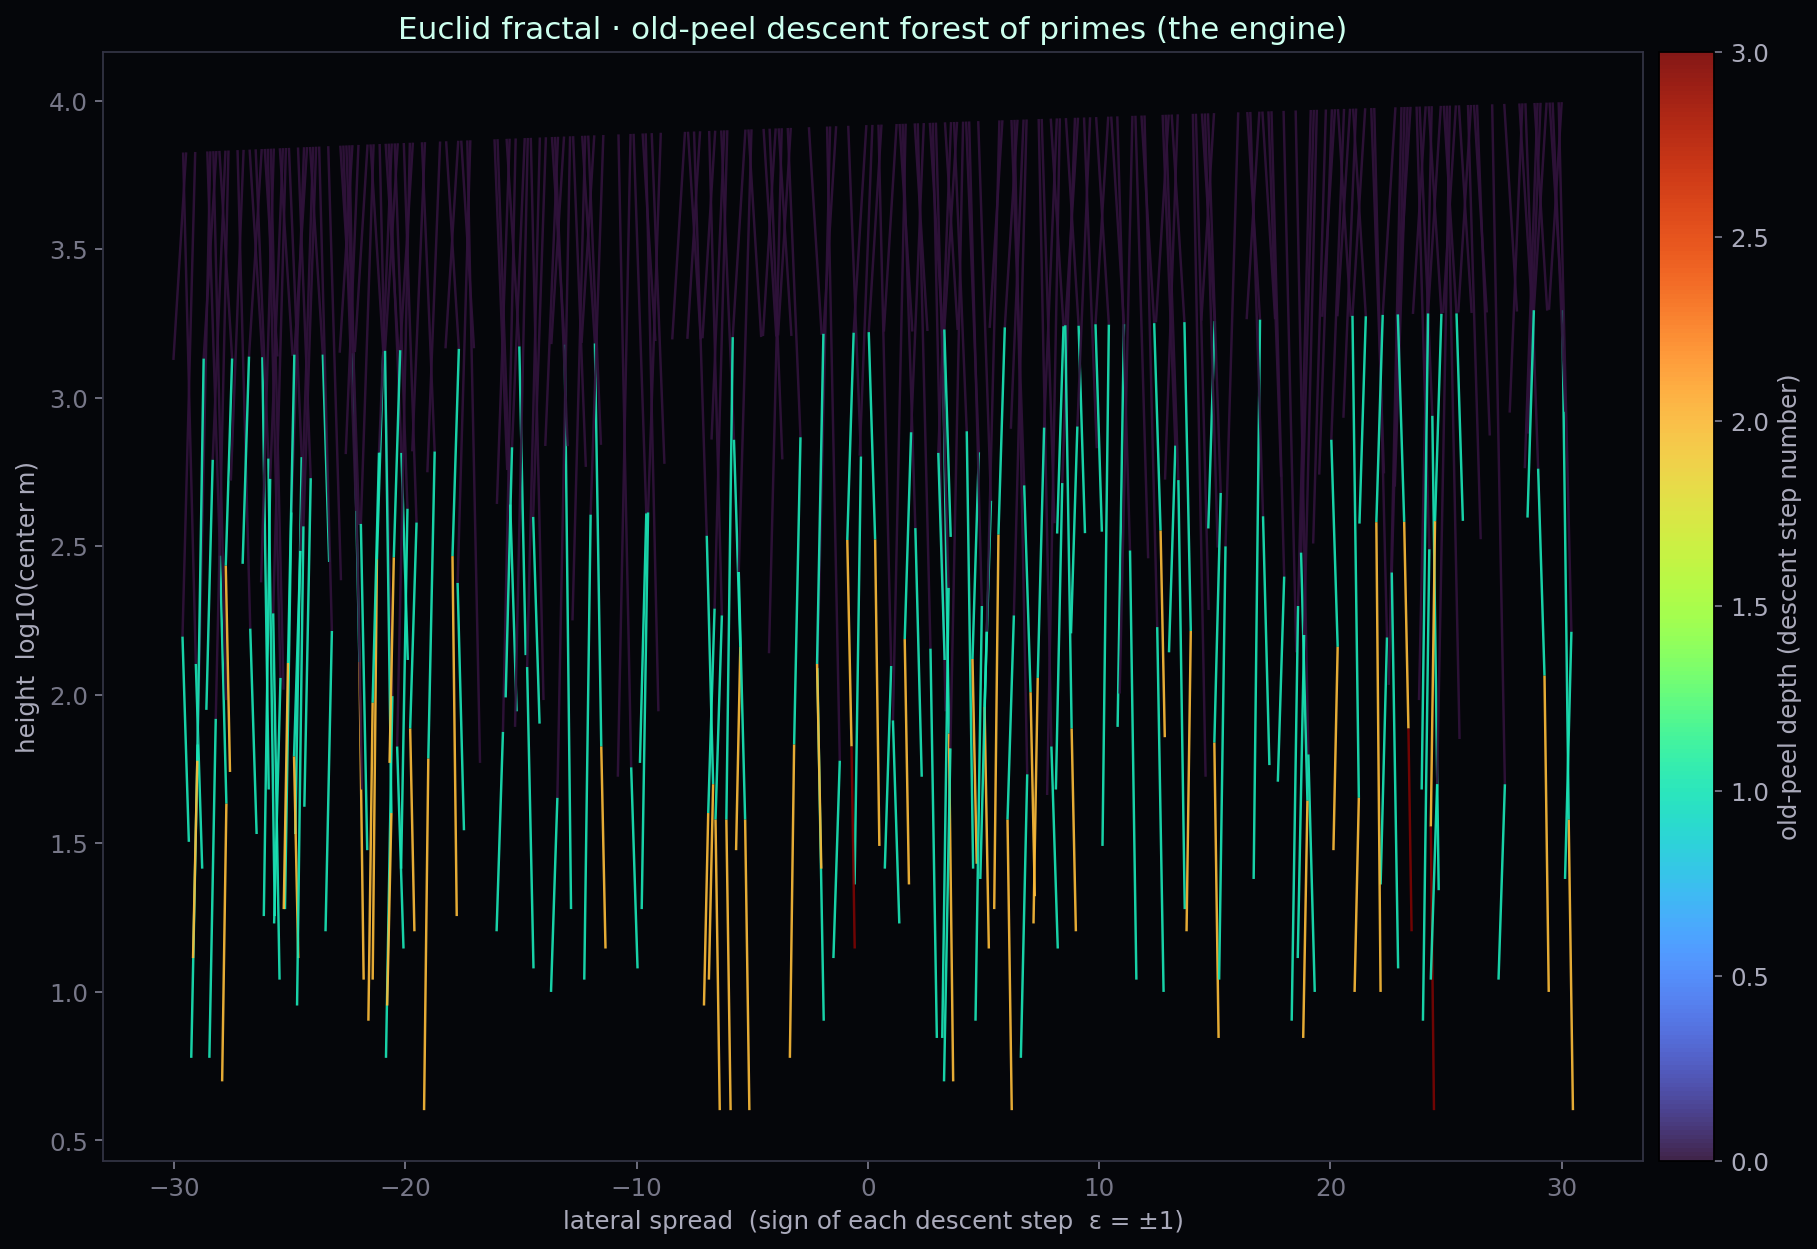
\includegraphics[width=\linewidth]{figures/1_old_peel_tree.png}
  \caption{The old-peel descent forest of primes --- the engine itself, run
  recursively from a row of large centres.}
  \label{fig:old-peel-tree}
\end{figure}

\emph{Generation algorithm (Figure~\ref{fig:old-peel-tree}).} Source:
\srcpath{tools/fractal/euclid\_fractal.py::old\_peel\_tree}. Fix $A=200$ and sieve
all primes up to $4A^2$; let the caught-prime pool be the primes $p$ with
$3<p\le A$. Seed a horizontal row of $460$ roots at abscissae $x$ evenly spaced
over $[-30,30]$, the $i$-th root carrying centre $n=\lfloor A^2/6\rfloor+7i$.
From each root run the recursive descent $\mathrm{peel}(n,\varepsilon,d,x)$ for
both signs $\varepsilon=\pm1$: it stops when depth $d>7$ or $n<2$; it requires
the side $a=6n+\varepsilon$ to be prime with $a>A$; it takes the opposite side
$6n-\varepsilon$, finds the first pool prime $p$ dividing it, forms the quotient
$q=(6n-\varepsilon)/p$, reads its sign $\delta$ from $q\bmod6$ ($\delta=+1$ if
$q\equiv1$, $\delta=-1$ if $q\equiv5$, aborting otherwise), and sets the child
centre $t=(q-\delta)/6$ (aborting if $t\le0$). The step draws a segment from
$(x,\ \log_{10}(n+1))$ to $(x+\varepsilon\cdot0.55/(d+1),\ \log_{10}(t+1))$, then
recurses into $t$ with both signs at depth $d+1$. The vertical axis is height
$\log_{10}(\text{centre})$; the horizontal offset encodes the descent sign
$\varepsilon$; segments are coloured by descent depth $d$ (turbo palette).

\begin{figure}[H]
  \centering
  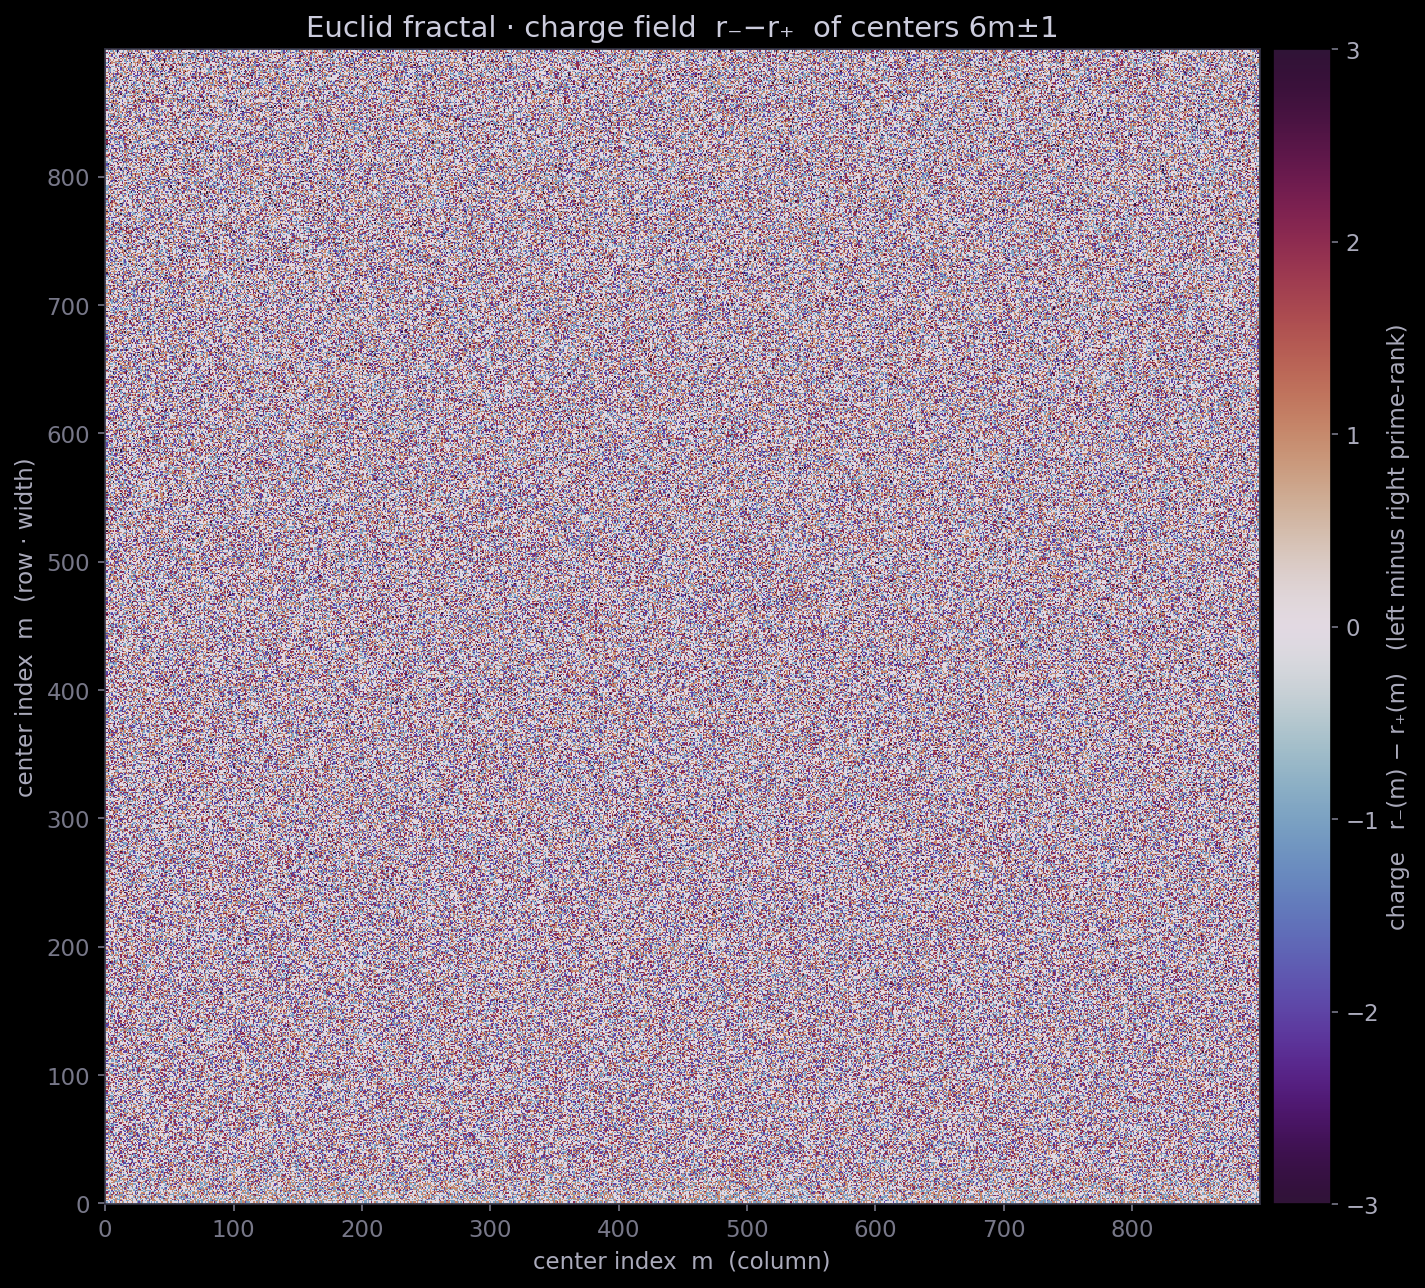
\includegraphics[width=\linewidth]{figures/2_rank_field.png}
  \caption{The charge field $r_-(m)-r_+(m)$ of the centres $6m\pm1$: the
  fractal generating function of prime rank.}
  \label{fig:rank-field}
\end{figure}

\emph{Generation algorithm (Figure~\ref{fig:rank-field}).} Source:
\srcpath{tools/fractal/euclid\_fractal.py::rank\_field}. Parameters $A=60$,
$W=900$; the prime layer is $\{p:\ A<p\le A^2\}$. For each centre index
$m\in\{0,\dots,W^2-1\}$ two ranks are counted: $r_-(m)$, the number of layer
primes dividing the lower side $6m-1$, and $r_+(m)$, the upper side $6m+1$. For
each $p$ the congruence $6m\equiv\pm1\pmod p$ is solved via the inverse
$6^{-1}\bmod p$, giving the root $r\equiv\pm6^{-1}\pmod p$, the start offset
$(r-1)\bmod p$, and a unit added to every $p$-th position of the array $r_\mp$.
The charge $r_-(m)-r_+(m)$ is imaged: the length-$W^2$ vector is reshaped into a
$W\times W$ matrix (row $=\lfloor m/W\rfloor$, column $=m\bmod W$) and drawn with
the diverging twilight-shifted palette (opposite charge signs at the two ends,
zero at the centre), lower origin.

\begin{figure}[H]
  \centering
  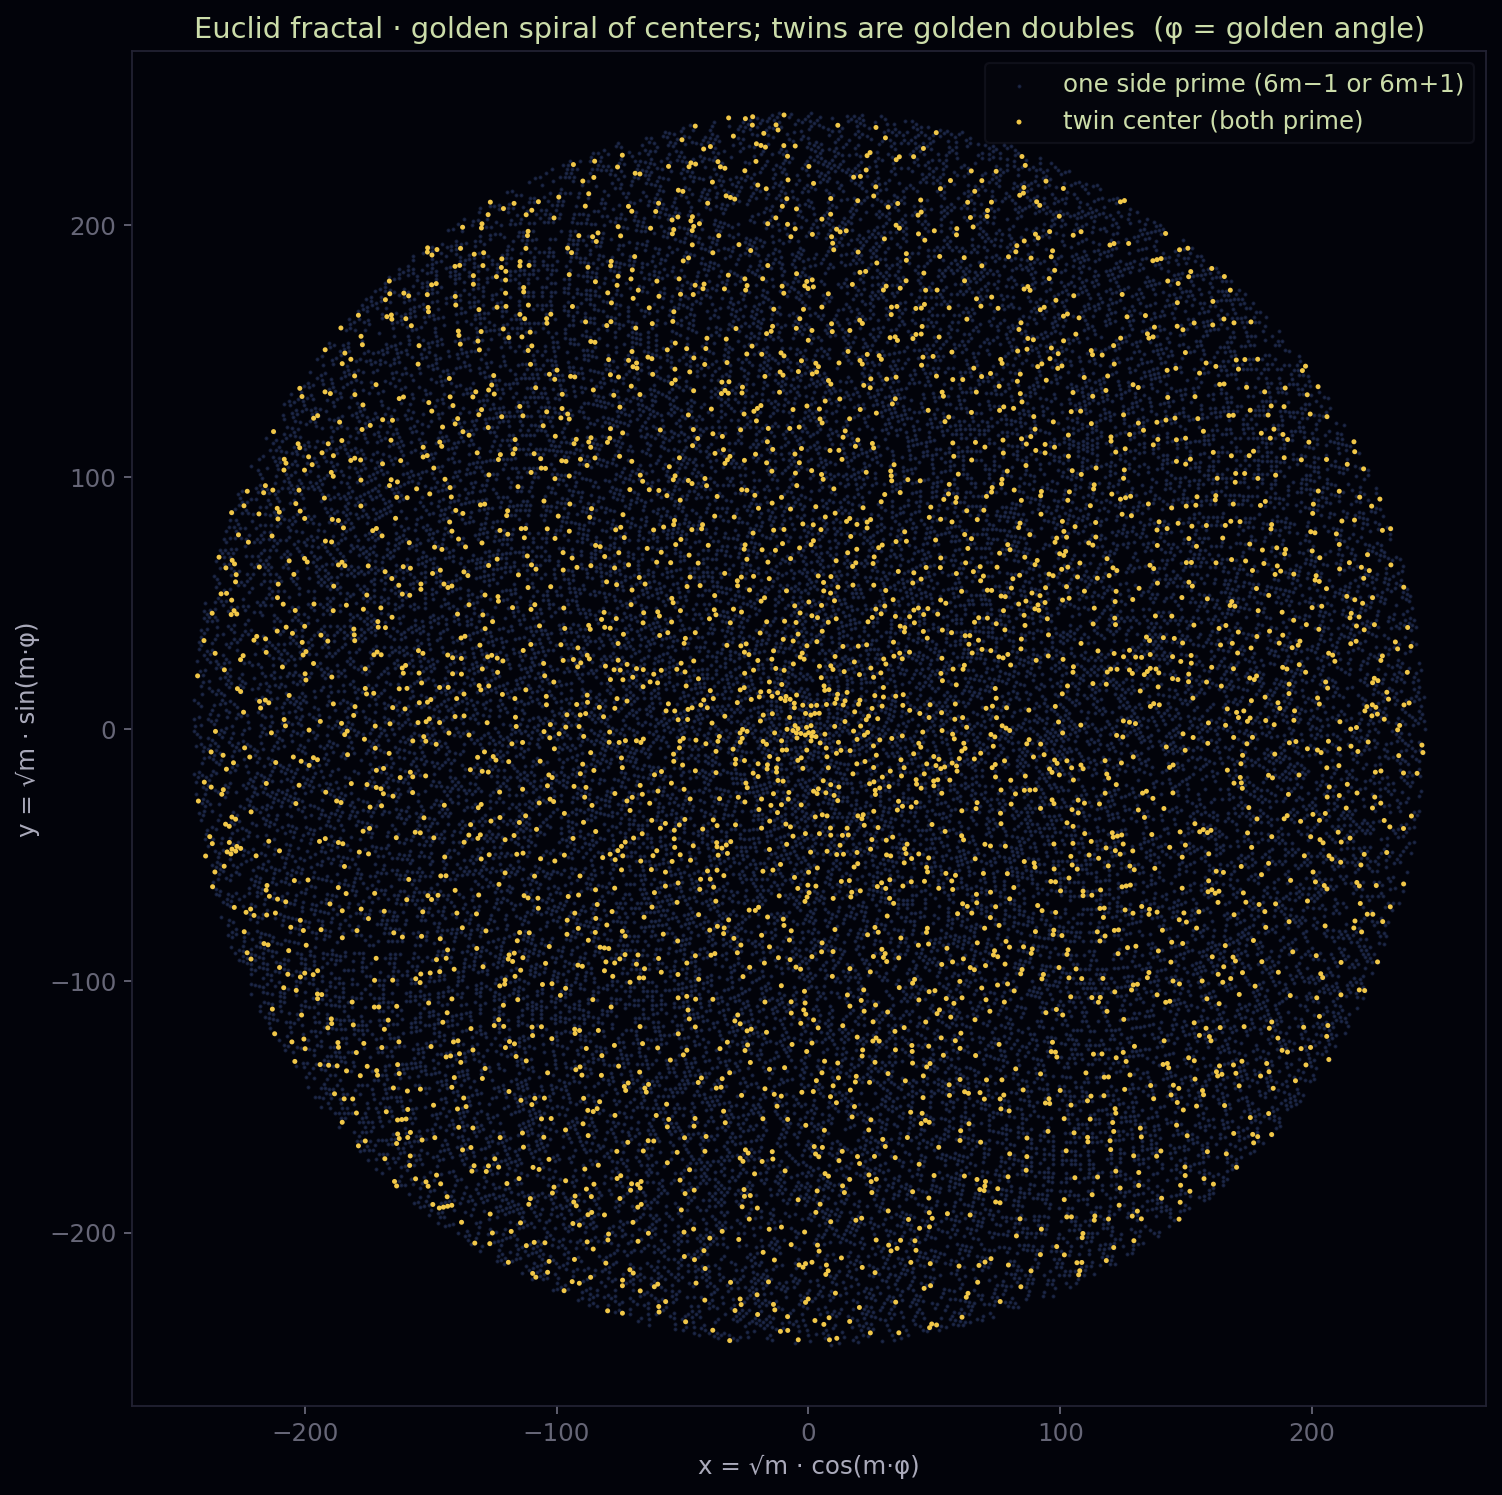
\includegraphics[width=\linewidth]{figures/3_twin_spiral.png}
  \caption{The golden spiral of centres; twin-centres are the golden doubles.}
  \label{fig:twin-spiral}
\end{figure}

\emph{Generation algorithm (Figure~\ref{fig:twin-spiral}).} Source:
\srcpath{tools/fractal/euclid\_fractal.py::twin\_spiral}. For each centre
$m=1,\dots,M-1$ (default $M=60000$) a point is placed on the golden spiral
\begin{equation}\label{eq:golden-spiral}
  x=\sqrt{m}\,\cos(m\varphi),\qquad
  y=\sqrt{m}\,\sin(m\varphi),\qquad
  \varphi=\pi(3-\sqrt5),
\end{equation}
with $\varphi$ the golden angle. A centre is marked one-sided prime when
$6m-1$ or $6m+1$ is prime (dim blue points), and a twin-centre when both sides
$6m\pm1$ are prime (large golden points). The radius $\sqrt m$ gives uniform
density per unit area; the colour is fixed per class.

\begin{figure}[H]
  \centering
  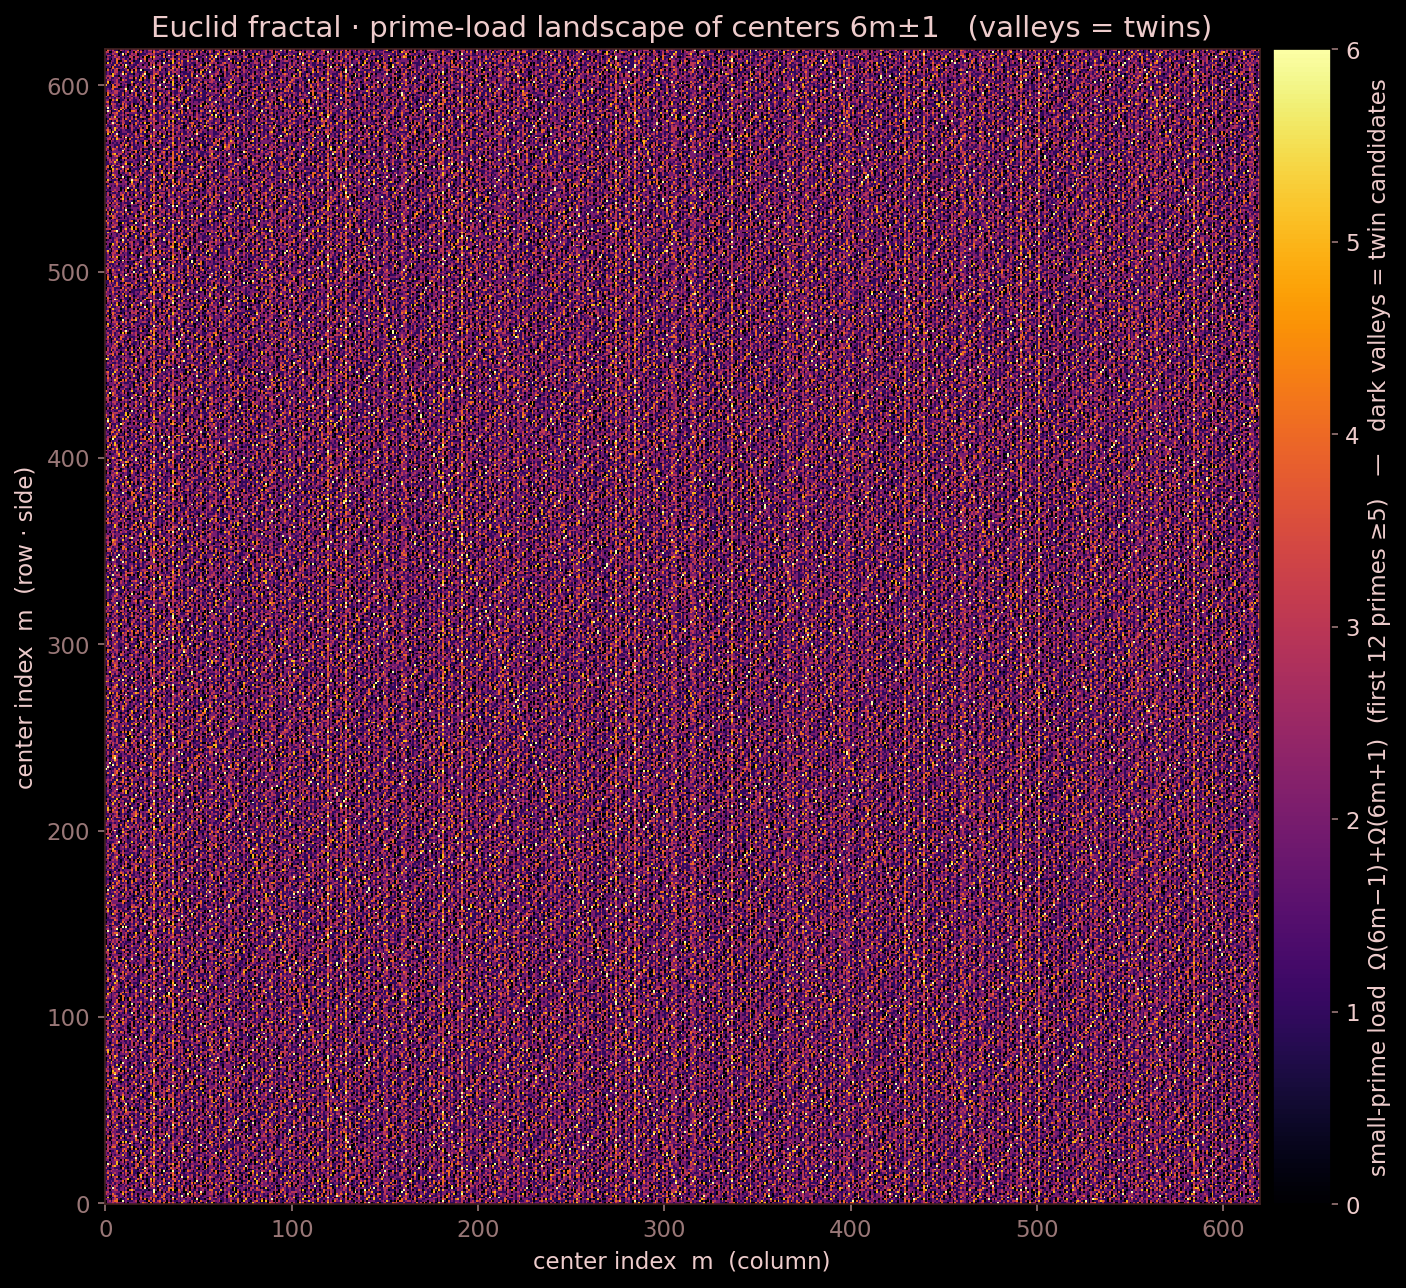
\includegraphics[width=\linewidth]{figures/4_descent_landscape.png}
  \caption{The prime-load landscape of the centres $6m\pm1$; the dark valleys
  are the twin candidates.}
  \label{fig:descent-landscape}
\end{figure}

\emph{Generation algorithm (Figure~\ref{fig:descent-landscape}).} Source:
\srcpath{tools/fractal/euclid\_fractal.py::descent\_landscape}. For every centre
$m=0,1,\dots,S^2-1$ laid on an $S\times S$ raster ($S=620$, row-major in $m$),
compute the small-prime load
\begin{equation}\label{eq:small-prime-load}
  L(m)\;=\;\Omega_B(6m-1)+\Omega_B(6m+1),
\end{equation}
where $\Omega_B(x)$ is the number of prime factors of $x$, counted with
multiplicity and restricted to the first $B=12$ primes $\ge5$ (that is,
$5,7,11,\dots,41$). Colour each cell by $L(m)$ (inferno palette, clipped at the
99th percentile). Twin centres --- where both sides $6m\pm1$ are prime --- have
$L(m)=0$ and appear as the dark valleys; the self-similar relief is the
Chinese-remainder periodicity of the small primes.

\begin{figure}[H]
  \centering
  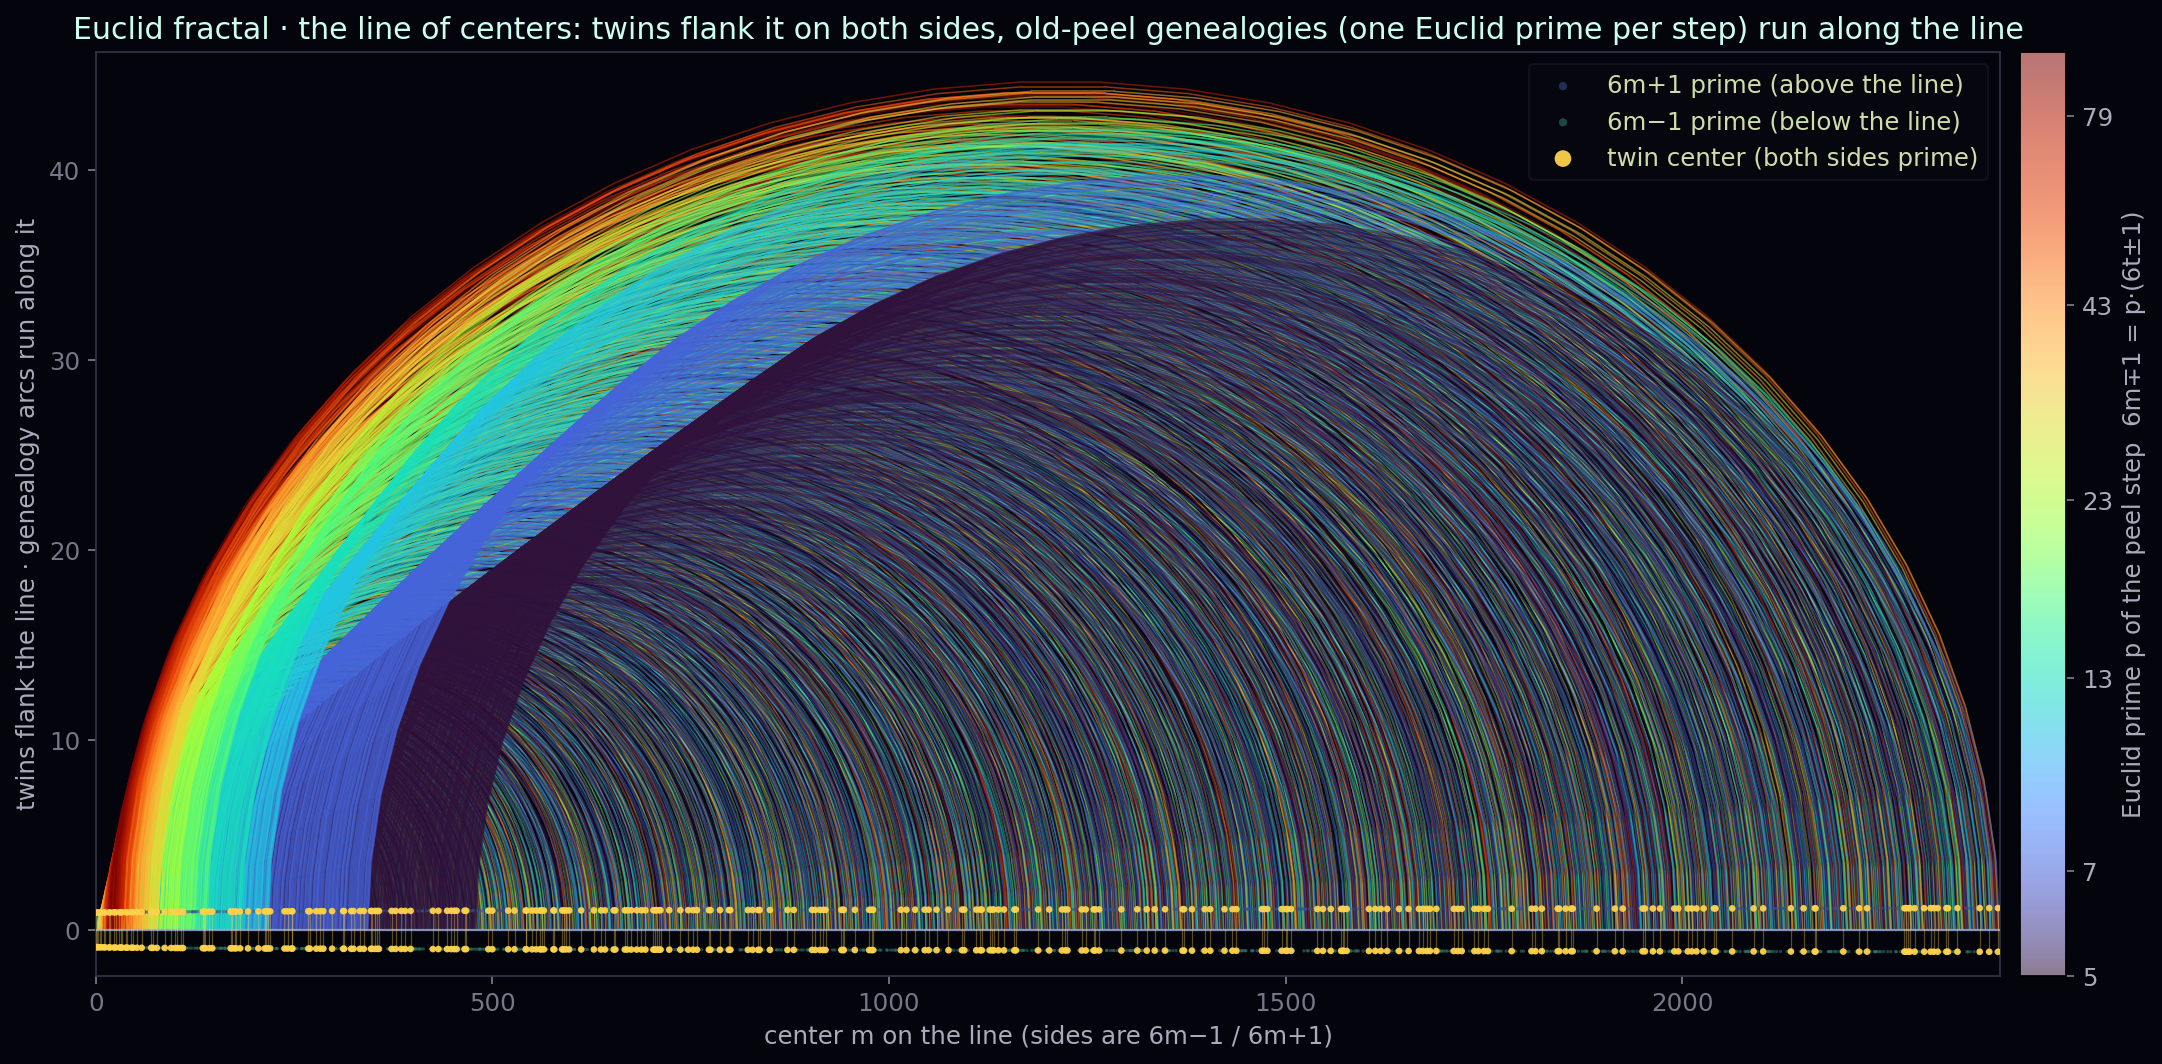
\includegraphics[width=\linewidth]{figures/5_twin_line_genealogy.png}
  \caption{The line of centres: twins flank it on both sides, old-peel
  genealogies (one Euclid prime per step) run along it.}
  \label{fig:twin-line-genealogy}
\end{figure}

\emph{Generation algorithm (Figure~\ref{fig:twin-line-genealogy}).} Source:
\srcpath{tools/fractal/euclid\_fractal.py::twin\_line\_genealogy}. Centres
$m=1,\dots,M$ ($M=2400$) are laid along the horizontal axis $y=0$. The side
$6m+1$ is marked by a point \emph{above} the line at height
$\mathrm{wing}(m)=0.9+0.25\sqrt{m/M}$, the side $6m-1$ by a symmetric point
below, whenever the corresponding number is prime (sieve to $6M+2$). A twin
centre (both sides prime) is marked by a golden vertical
$[-\mathrm{wing},\,+\mathrm{wing}]$ with points at its ends. Along the line, for
each $m$ the old-peel step is computed: if $6m\mp1=p\,(6t\pm1)$ with a Euclid
witness prime $p\in[5,97]$, a semicircular arc $m\to t$ is drawn of height
$h=0.06\,|m-t|^{0.85}+0.4$ (36 points,
$x=\tfrac{m+t}{2}+\tfrac{|m-t|}{2}\cos\theta$, $y=h\sin\theta$,
$\theta\in[0,\pi]$), coloured by $\log p$ (turbo palette). Twin centres live
\emph{off} the line, the genealogy \emph{on} it.

\begin{figure}[H]
  \centering
  \includegraphics[width=\linewidth]{figures/6_genealogy_ornament.png}
  \caption{The genealogy ornament: the full old-peel descent of every centre,
  woven as chords on the circle of centres.}
  \label{fig:genealogy-ornament}
\end{figure}

\emph{Generation algorithm (Figure~\ref{fig:genealogy-ornament}).} Source:
\srcpath{tools/fractal/euclid\_fractal.py::genealogy\_ornament} ($M=4200$,
$\mathrm{PMAX}=97$, $\mathrm{DEPTH}=10$). Centres $1,\dots,M$ sit on the unit
circle at angle $2\pi m/M$. For each centre the full old-peel genealogy
$m\to t_1\to t_2\to\cdots$ (to depth $10$) is built by the step
$6k\mp1=p\,(6t\pm1)$: each step is a Bézier chord with control point
$\tfrac12(P_a+P_b)\cdot(1-0.92\min(2\Delta\theta,1))$, where
$\Delta\theta=|a-b|/M$ (long chords dive deeper toward the centre); colour by
$\log p$ (turbo). Twin-centres (empty genealogy) sit on the rim as golden
points.

The two remaining figures are conceptual: they place the \emph{real}
genealogy in a cosmological picture. We stress the honest boundary, exactly as
in the coda: only the irreversibility of time and the curvature of space are
rigorously proved (the engine impossibility of \cref{sec:engine}); the reading
of the pictures as physics is a translation, not a theorem.

\begin{figure}[H]
  \centering
  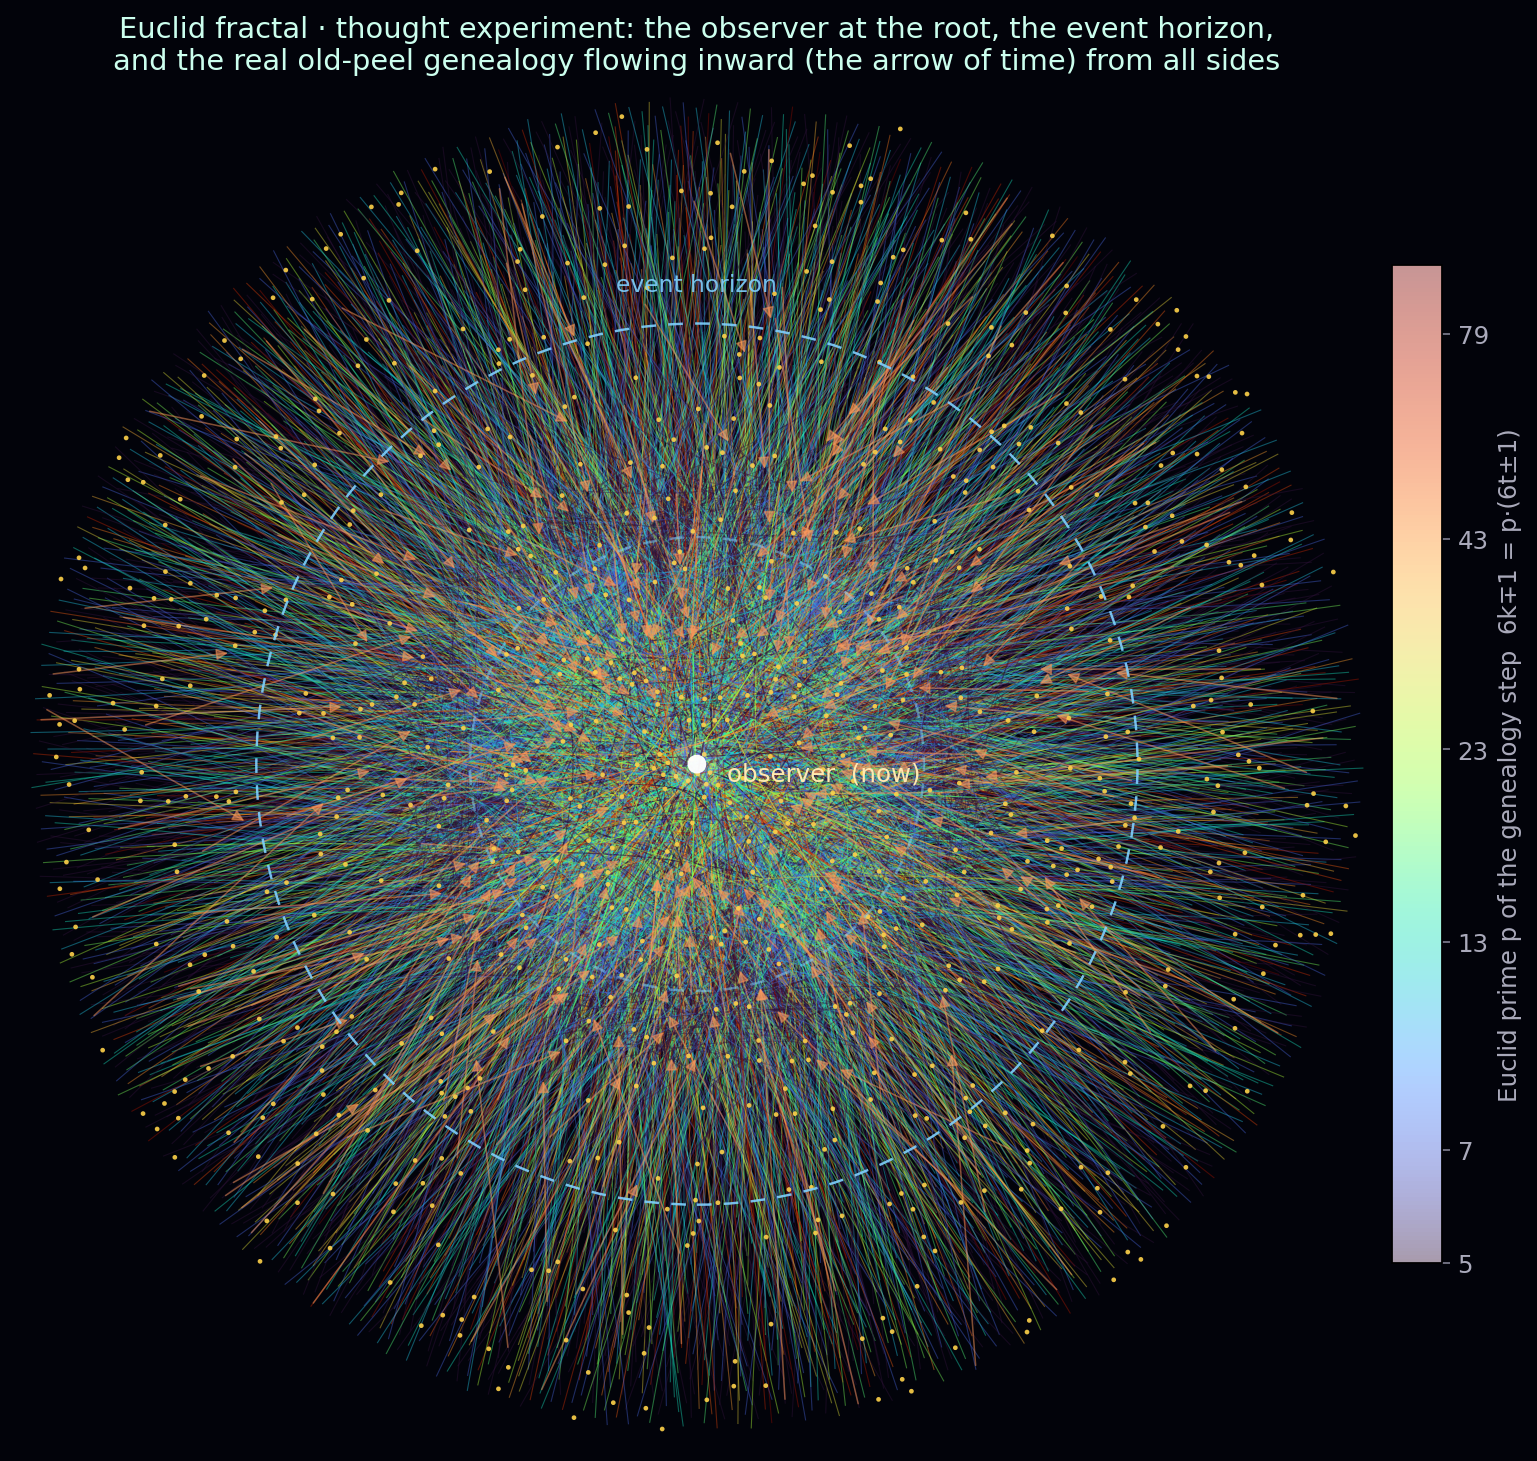
\includegraphics[width=\linewidth]{figures/7_observer_horizon.png}
  \caption{Thought experiment: the observer at the root, the event horizon, and
  the real old-peel genealogy flowing inward (the arrow of time).}
  \label{fig:observer-horizon}
\end{figure}

\emph{Generation algorithm (Figure~\ref{fig:observer-horizon}).} Source:
\srcpath{tools/fractal/euclid\_cosmology.py::observer\_horizon} ($M=9000$,
$\mathrm{PMAX}=97$, $\mathrm{DEPTH}=9$). Centre $k$ is placed on a golden spiral
by radius-height $r=\sqrt{k/M}$ and angle $k\varphi$ ($\varphi$ the golden
angle): small $k$ near the centre (the observer), large $k$ on the periphery.
The full old-peel genealogy of each centre is built by the step
$6k\mp1=p\,(6t\pm1)$ (smallest prime divisor $p\in[5,97]$ of the composite side,
$t<k$), iterated to depth $9$. Each step $k\to t$ is drawn as a quadratic Bézier
with control point $\tfrac12(P_k+P_t)\cdot0.72$ pulled toward the origin (the arc
dives inward); colour by $\log p$ (turbo palette). Orange arrows are placed on
real first steps with $r>0.30$ and point from $k$ to $t$ (inward). The dashed
circles of radius $0.66$ and $0.34$ are the event horizon; golden dots are
twin-centres.

\begin{figure}[H]
  \centering
  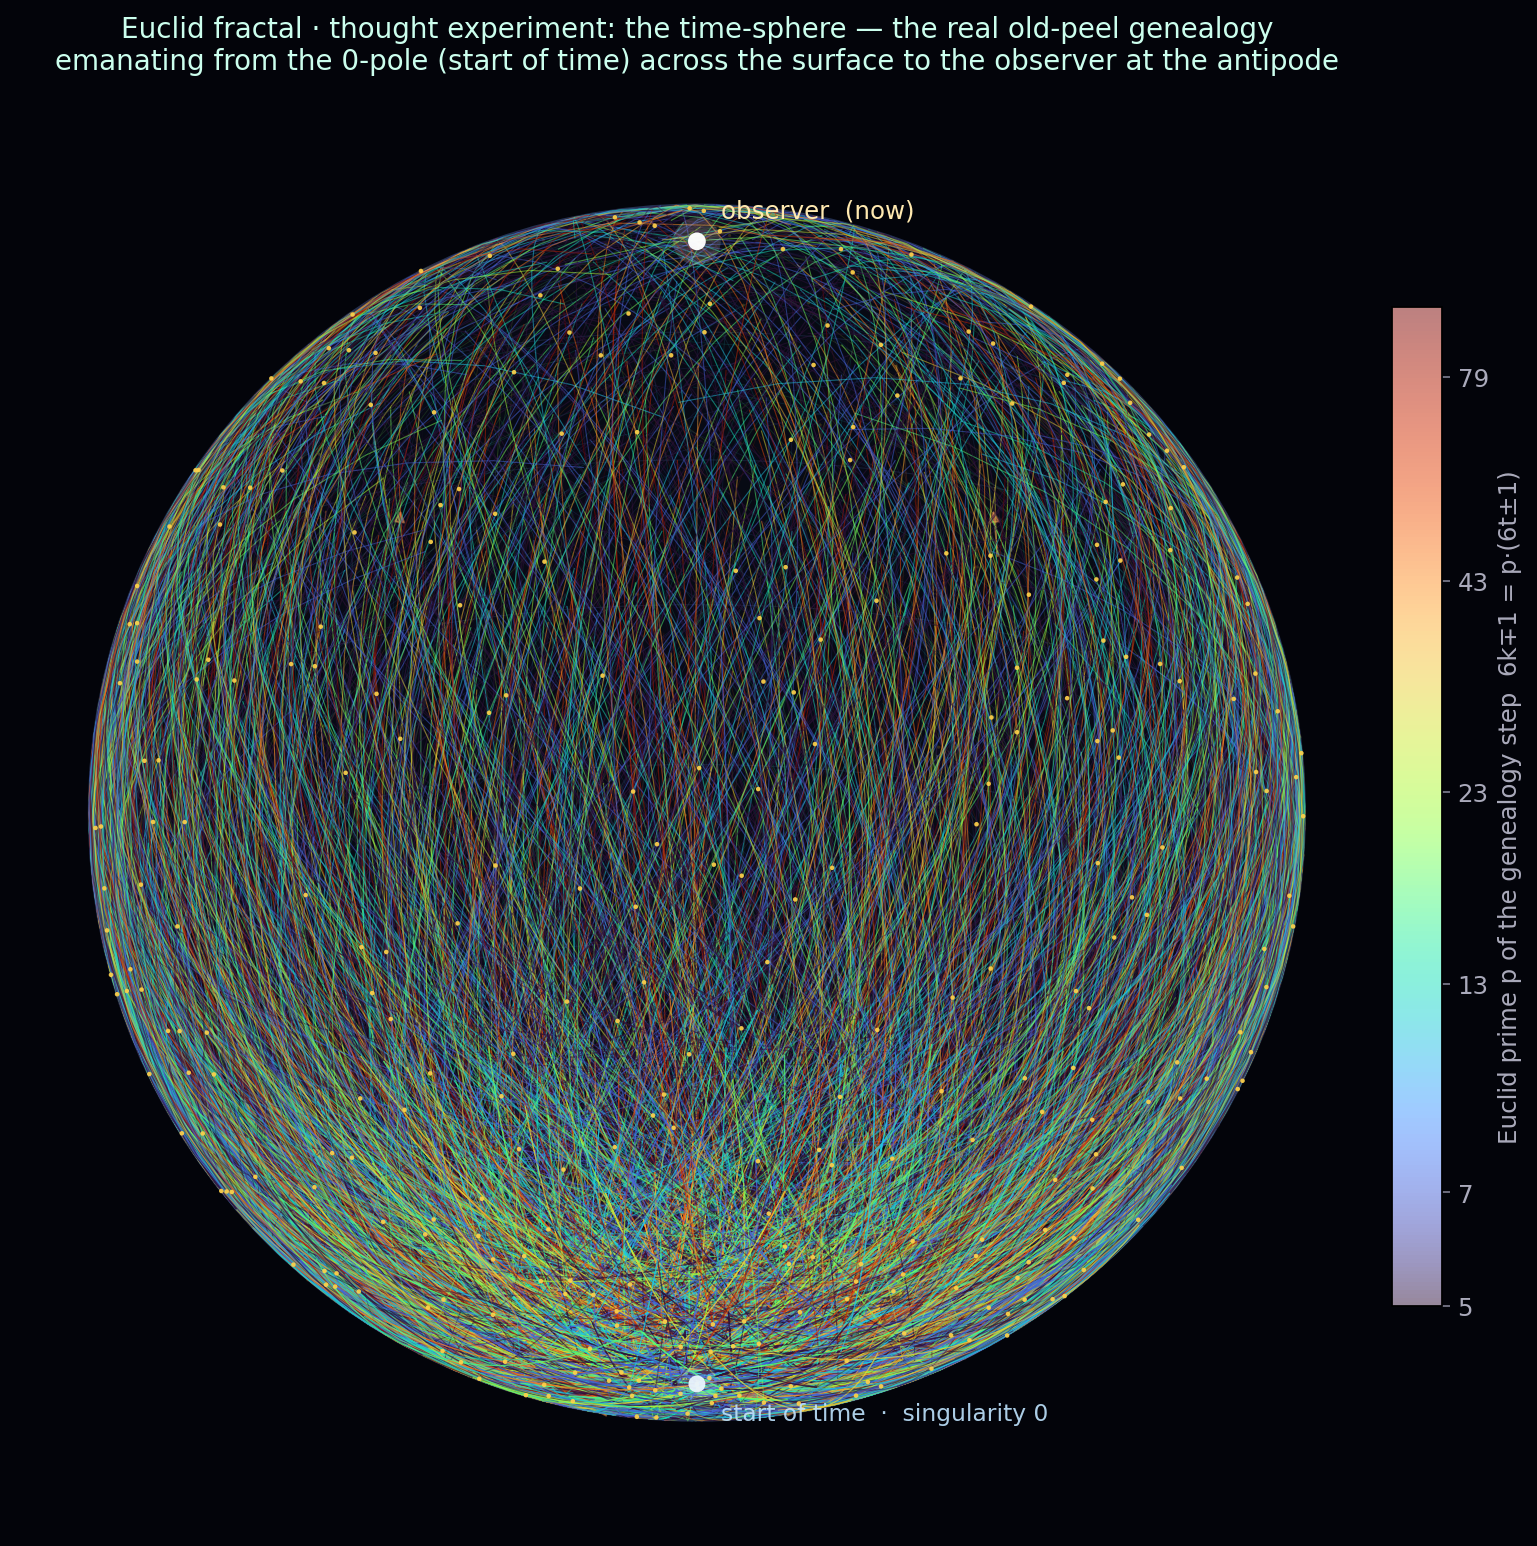
\includegraphics[width=\linewidth]{figures/8_time_sphere.png}
  \caption{Thought experiment: the time-sphere --- the real old-peel genealogy
  emanating from the $0$-pole (start of time) to the observer at the antipode.}
  \label{fig:time-sphere}
\end{figure}

\emph{Generation algorithm (Figure~\ref{fig:time-sphere}).} Source:
\srcpath{tools/fractal/euclid\_cosmology.py::time\_sphere} ($M=7000$,
$\mathrm{PMAX}=97$, $\mathrm{DEPTH}=9$). Centre $k$ maps to a unit vector on the
sphere: height $z=-1+2(k-1)/(M-1)$ (so $k=1$ is at the $0$-pole, $z=-1$; $k=M$ at
the observer-pole, $z=+1$), longitude $k\varphi$ by the golden angle,
$\rho=\sqrt{1-z^2}$. The full old-peel genealogy $6k\mp1=p\,(6t\pm1)$ (depth $9$)
is drawn as great-circle arcs (spherical slerp between $V_k$ and $V_t$);
front-hemisphere arcs bright, back-hemisphere faint; colour by $\log p$ (turbo).
The projection is a $20^\circ$ rotation about the $x$-axis. Orange meridian
arrows mark the generative direction of time from the $0$-pole to the
observer-pole; golden dots are twin-centres; the two poles are labelled
``observer (now)'' and ``start of time $\cdot$ singularity $0$''.
